\documentclass[10pt,a4paper]{article}

% ------------------------------------------------------------------ fonts and layout
\usepackage[T1]{fontenc}
\usepackage[utf8]{inputenc}
\usepackage{newtxtext,newtxmath}
\usepackage[scaled=0.86]{beramono}
\usepackage[margin=2.3cm,top=2.4cm,bottom=2.5cm]{geometry}
\usepackage{microtype}
\usepackage{graphicx}
\usepackage{float}
\usepackage{xurl}
\usepackage{booktabs,tabularx,longtable,multirow,array}
\usepackage{threeparttable}
\usepackage[table]{xcolor}
\usepackage{caption,subcaption}
\usepackage{enumitem}
\usepackage{amsmath}
\usepackage{siunitx}
\usepackage[ruled,vlined,linesnumbered]{algorithm2e}
\usepackage[most]{tcolorbox}
\usepackage{fancyhdr}
\usepackage{titlesec}
\usepackage[hidelinks]{hyperref}
\usepackage[nameinlink,capitalise]{cleveref}

\definecolor{almablue}{HTML}{1D4E89}
\definecolor{almaorange}{HTML}{C2410C}
\definecolor{softgrey}{HTML}{F3F5F8}
\definecolor{goodgreen}{HTML}{E6F4EA}
\definecolor{warnamber}{HTML}{FDF3E1}
\definecolor{badred}{HTML}{FBE9E9}

\captionsetup{font=small,labelfont={bf,color=almablue},skip=4pt}
\setlist{itemsep=1.5pt,topsep=3pt,leftmargin=1.4em}
\titleformat{\section}{\large\bfseries\color{almablue}}{\thesection}{0.6em}{}
\titleformat{\subsection}{\normalsize\bfseries}{\thesubsection}{0.6em}{}
\titleformat{\subsubsection}{\normalsize\itshape}{\thesubsubsection}{0.6em}{}
\titlespacing*{\section}{0pt}{12pt}{5pt}
\titlespacing*{\subsection}{0pt}{8pt}{3pt}
\renewcommand{\arraystretch}{1.12}
\sisetup{detect-all}

\pagestyle{fancy}
\fancyhf{}
\fancyhead[L]{\small\color{gray}Alma Models: Project Status Report}
\fancyhead[R]{\small\color{gray}3 November 2026}
\fancyfoot[C]{\small\thepage}
\renewcommand{\headrulewidth}{0.3pt}

\newtcolorbox{keybox}[1][]{colback=softgrey,colframe=almablue!60,boxrule=0.5pt,arc=1.5pt,left=6pt,right=6pt,top=4pt,bottom=4pt,fonttitle=\bfseries\small,#1}
\newtcolorbox{goodbox}[1][]{colback=goodgreen,colframe=green!35!black!40,boxrule=0.5pt,arc=1.5pt,left=6pt,right=6pt,top=4pt,bottom=4pt,fonttitle=\bfseries\small,#1}
\newtcolorbox{badbox}[1][]{colback=badred,colframe=red!50!black!40,boxrule=0.5pt,arc=1.5pt,left=6pt,right=6pt,top=4pt,bottom=4pt,fonttitle=\bfseries\small,#1}
\newcommand{\src}[1]{{\footnotesize\texttt{#1}}}
\newcommand{\yes}{\textcolor{green!45!black}{\textbf{yes}}}
\newcommand{\no}{\textcolor{red!60!black}{\textbf{no}}}
\newcommand{\new}[1]{\textcolor{almaorange}{\textbf{#1}}}

\begin{document}

% ------------------------------------------------------------------ title page
\begin{titlepage}
\thispagestyle{empty}\setlength{\parindent}{0pt}
\vspace*{2.2cm}
{\color{almablue}\rule{\linewidth}{1.2pt}}\\[0.6cm]
{\Huge\bfseries Alma Models}\\[0.35cm]
{\LARGE Project Status Report}\\[0.25cm]
{\large Verified results, independent audit, improvements, benchmarks and roadmap}\\[0.4cm]
{\color{almablue}\rule{\linewidth}{1.2pt}}\\[1.2cm]

\noindent\begin{tabularx}{\linewidth}{@{}lX@{}}
\textbf{Report date} & 3 November 2026 (covers the project from its first goal draft, 29 October 2026, to today)\\
\textbf{Repository} & \url{https://github.com/Bhavith-Chandra/Alma-Models}, branch \texttt{main} at commit \texttt{43b463b}\\
\textbf{Prepared by} & Claude Code (model Claude Opus 5.5), working on the project owner's machine\\
\textbf{Status of this document} & Every number was read from a result file in the repository or the audit folder, or recomputed for this report; \cref{app:provenance} maps each number to its source file.\\
\end{tabularx}

\vspace{1.2cm}
\noindent\begin{keybox}[title=How to read this report]
\begin{itemize}
\item \textbf{Repo-reported} numbers come from the project's own sealed TEST runs (\src{repo/runs/*/test/}), which the project's internal auditor re-derived.
\item \textbf{Re-verified} numbers were recomputed independently in the audit of 1 November 2026, with separate scoring code.
\item \textbf{New} (shown in \new{orange}) marks models and results created by the audit. Their TEST scores are a \emph{second look} at a test year the project had already scored, so they are indicative until the forward test confirms them.
\item ``Significant'' always means a 95\% confidence interval (or a Holm-corrected $p<0.05$, where stated) that excludes no difference. Results that are only numerically better are called that.
\end{itemize}
\end{keybox}
\vfill
{\small\color{gray} Hardware used for all project training: one 8\,GB Apple M3 MacBook (as stated in the repository README).}
\end{titlepage}

% ------------------------------------------------------------------ abstract
\begin{abstract}
\noindent Alma is a family of time-series \emph{world models}: a latent state is advanced step by step by a learned transition, and forecasts are read out from the simulated states. The project has four completed market studies (WTI crude oil, German day-ahead power, US natural-gas storage and crypto volatility), each evaluated once on a sealed, pre-registered TEST year (November 2025 to October 2026). It also has a live gas paper-trading study in progress and a zero-shot research track aimed at public benchmarks. An independent audit rebuilt the data from public sources, re-ran every frozen checkpoint with separate scoring code, and ran leak tests that scramble all future information. \textbf{No data leakage and no fabricated numbers were found}: the four headline TEST results reproduce. Several headline \emph{claims} were stronger than the evidence, and these were corrected. The central scientific hypothesis, that the learned rollout beats an otherwise identical direct decoder, \textbf{is not supported in any project}, including the research-track SSM over five seeds. Seed ensembles and quantile blends with the strongest simple baseline, all chosen on development data, improved gas storage (MAE 10.63 vs 11.53\,Bcf), power (quantile score 8.60 vs 9.03) and crypto volatility (direction accuracy 0.740 vs 0.724 under the same rule). None of the three significantly beats its best simple baseline on direction. On the zero-shot track, Alma (bench-VAL wql\_rel 0.6806, 5-seed mean) remains well behind Chronos-2 (0.559) and Timestral-5M (0.585), and there is no fev-bench score yet. A forward test frozen on 1 November 2026 will score the improved models on data that did not exist when they were built. The first data arrive on 5 November 2026; confirming the main gains statistically will take between a few months and several years, depending on the comparison (\cref{sec:projection}).
\end{abstract}

\tableofcontents
\clearpage

% ================================================================== 1
\section{Status at a glance}
\label{sec:glance}

\begin{table}[H]
\centering\small
\caption{Overall project status on 3 November 2026.}
\label{tab:glance}
\begin{tabularx}{\linewidth}{@{}p{3.6cm}p{2.6cm}X@{}}
\toprule
Work stream & Status & Verified state\\
\midrule
1. Oil (WTI) & Done, audited & TEST reproduced exactly. 1-day probabilistic forecast ties the random walk (skill +0.45\%, $p=0.479$).\\
2. Power (Germany) & Done, audited & TEST reproduced. Hourly direction 0.747 is numerically first but not significantly better than LEAR, ARX or the foundation models.\\
3. Gas storage (EIA) & Done, audited & TEST reproduced exactly. Best quantile score of all external models (significant vs OLS and the foundation models).\\
4. Crypto volatility & Done, audited & TEST reproduced. Beats Chronos-2, TiRex, Chronos-Bolt and Kronos on quantile score; ties the weekday HAR baseline on direction.\\
5. Alma-Live Gas & In progress & Harness, data pins and 8 shadow paper-trading baselines exist (ledgers started 2026-11-01). No world-model result has been recorded yet.\\
Zero-shot research track & In progress & Bench-VAL wql\_rel 0.6806 (5-seed mean) vs Chronos-2 0.559. fev-bench run paused: 7 of 52 eligible tasks predicted, no skill score.\\
World-model hypothesis & \textbf{Not supported} & The matched direct twin is equal or better on TEST in every project, and the SSM rollout gain over 5 seeds is not significant.\\
Integrity audit & Done & No leaks (oil 0/25, gas 0/26, power 0/25 forecasts changed under future scrambling; the new wm\_gas\_ens 0/22); no fabricated numbers.\\
Improvements & Done (\new{new}) & Gas ensemble, power blend and crypto blend packaged with checksum-checked wrappers.\\
Forward test & Frozen, waiting for data & 29 files pinned at 2026-11-01 17:47 UTC; first gas data 2026-11-05.\\
Code & Merged & Audit fixes merged into GitHub \texttt{main} (merge commit \texttt{43b463b}).\\
\bottomrule
\end{tabularx}
\end{table}

\begin{goodbox}[title=What went well]
\begin{itemize}
\item The evaluation protocol is sound: pre-registration, sha256 pins, single TEST look and information-set checks. Every headline number survived an independent rebuild.
\item Gas storage is a genuine win on probabilistic accuracy: wm\_gas has the best quantile score of all external models, and the audit ensemble lowers MAE to 10.63\,Bcf.
\item Cheap, honest improvements worked in three projects without touching TEST for selection.
\end{itemize}
\end{goodbox}
\begin{badbox}[title=What went wrong]
\begin{itemize}
\item The defining idea (rollout beats a direct decoder) failed its own test everywhere.
\item Some headline claims were framed too favourably (oil ``\#1 of 9'', the crypto ``transfer to unseen coins'' claim and the SSM ``first to pass'' claim). These are now corrected.
\item The zero-shot model is about 22\% worse than Chronos-2 on the internal bench, and the public-benchmark run stopped because of an out-of-memory situation on the 8\,GB machine.
\item In crypto, the RL trading agent lost to DQN, and there was no ETF transfer.
\end{itemize}
\end{badbox}

% ================================================================== 2
\section{Project goal and success criteria}
\label{sec:goal}

The goal document (\src{repo/alma\_goal.md}, draft v1 of 31 October 2026) states the mission as \emph{``Building the World's Most Accurate, Efficient, and Generalizable World Models for Time-Series Forecasting''}. It also sets a mandatory scientific test and three accuracy tiers on the public benchmarks fev-bench and GIFT-Eval.

\paragraph{The world-model test (mandatory).} Alma must beat an otherwise identical \emph{direct} model (same encoder, parameters, data and compute, decoding the horizon in one shot without a state rollout) on the primary metric over at least 3 seeds, with a paired bootstrap CI excluding 0. If the direct model wins or ties, the result does not count as a world-model result.

\begin{table}[H]
\centering\small
\caption{Success tiers from \src{alma\_goal.md} \S4 and today's status. SQL skill is fev-bench (higher is better); rel.\ CRPS is GIFT-Eval (lower is better). Leaderboard values are as recorded in the goal document.}
\label{tab:tiers}
\begin{tabularx}{\linewidth}{@{}lXl@{}}
\toprule
Tier & Requirement (both benchmarks, significant after Holm) & Status today\\
\midrule
Full goal & Beat every model, incl.\ Timestral-209M (50.4 / 0.446) and the current fev \#1 (TimeRSI-1.5, 51.8) & Not met; no score yet\\
Strong & Beat Chronos-2 (47.3 / 0.485) and Timestral-28M (48.4 / 0.461) & Not met; no score yet\\
Minimum & Beat Timestral-5M (46.2 / 0.479) and TiRex (42.6 / 0.488) & Not met; no score yet\\
World-model test & Rollout beats direct twin, $\geq$3 seeds, CI excludes 0 & \textbf{Failed} (SSM, 5 seeds; \cref{sec:wm})\\
\bottomrule
\end{tabularx}
\end{table}

The four market projects are a separate track. Each has its own pre-registration (\src{docs/*\_prereg.md}) and asks whether a domain world model beats statistical baselines and foundation models on a sealed TEST year.

% ================================================================== 3
\section{Timeline of work}
\label{sec:timeline}

\begin{table}[H]
\centering\small
\caption{Dated milestones, taken from the documents, run files and git history.}
\label{tab:timeline}
\begin{tabularx}{\linewidth}{@{}p{3.4cm}X@{}}
\toprule
Date (2026) & Event\\
\midrule
29--31 Oct & Mission and goal drafted (\src{alma\_goal.md}); research history reconciled (\src{docs/research\_history.md}, 269 ledger rows).\\
31 Oct 20:00 EDT & Oil TEST scored once (commit \texttt{97be9e5}).\\
31 Oct 22:06 EDT & Power TEST scored once (commit \texttt{652621f}).\\
31 Oct & fev-bench run paused for a memory emergency (\src{docs/fev\_full\_results.md}).\\
1 Nov 00:30 EDT & Gas TEST scored once (commit \texttt{fed026b}).\\
1 Nov 05:31 EST & Crypto TEST scored once (commit \texttt{90a86c2}).\\
1 Nov 08:44 EST & Repository published (commit \texttt{731edfa}).\\
1 Nov 12:56 UTC & Alma-Live shadow paper ledgers started (genesis entries in \src{runs/live/paper/anchors.log}).\\
1 Nov & Independent audit: data rebuilt, checkpoints re-scored, leak tests, improvement experiments.\\
1 Nov 16:34 / 17:00 UTC & Gas candidate and interval rule frozen in writing before any TEST score of them (\src{audit/GAS\_FREEZE.md}).\\
1 Nov 17:47 UTC & Forward test frozen (29 pinned files).\\
1 Nov & 8 research-track runs trained for the 5-seed SSM test; audit commits \texttt{9f96b36} and \texttt{7f8c068}.\\
1 Nov (pushed) & Audit fixes merged into \texttt{main} on GitHub (\texttt{43b463b}).\\
3 Nov & This report; all audit scoring scripts re-run and their outputs saved (\src{audit/validation/}).\\
5 Nov (planned) & First forward-test data point (EIA weekly storage report).\\
\bottomrule
\end{tabularx}
\end{table}

% ================================================================== 4
\section{Evaluation protocol}
\label{sec:protocol}

\begin{table}[H]
\centering\small
\caption{Prediction targets, TEST windows and metrics (from the pre-registrations and TEST reports).}
\label{tab:protocol}
\begin{tabularx}{\linewidth}{@{}p{2.1cm}Xp{3.2cm}p{3.6cm}@{}}
\toprule
Project & Target & TEST window & Primary metrics\\
\midrule
Oil & WTI log price at $h=1,5,20$ days (direction and quantiles) & 246 origins, 2025-11-03 to 2026-10-27 & Quantile score (QS), direction\\
Power & German day-ahead price, 24 hours (DE-LU) & 365 days, 2025-11-01 to 2026-10-31 & P1 daily, P2 hourly, P3 spread direction; P4 QS\\
Gas & Weekly EIA storage change, Lower 48 (+5 regions), Thursday and Friday origins & 52 weeks, 2025-10-31 to 2026-10-23 & MAE (Bcf), QS, direction vs 5-yr average\\
Crypto & Next-day 5-min realized-vol direction (P1), log-RV quantiles (P3); trading Sharpe (P2) & 2025-11-01 to 2026-10-30; 16 training + 8 held-out coins & P1 accuracy, P3 QS, net Sharpe\\
\bottomrule
\end{tabularx}
\end{table}

\paragraph{Metrics.} The quantile score is the mean pinball loss over the forecast quantiles: for level $\tau$ and outcome $y$, $\rho_\tau(y-\hat q_\tau)=\max\{\tau(y-\hat q_\tau),(\tau-1)(y-\hat q_\tau)\}$. Lower is better, and the score rewards both accuracy and calibration. Coverage is the share of outcomes inside the central 80\% (or 95\%) interval, ideally 0.80 (0.95). Direction accuracy is the share of correct up/down calls relative to the task's reference (previous value, 5-year average, or trailing 7-day mean log-volatility).

\paragraph{Statistics.} The project uses Diebold--Mariano tests with the HLN correction, block-bootstrap confidence intervals and Holm correction over competitors. The audit used day- or week-block bootstraps (4,000 replicates) and, for the research bench, a family-cluster bootstrap over 13 task families.

\paragraph{Integrity controls.} Each project has a dated pre-registration and amendments. Data and checkpoints are pinned by sha256. The strict TEST mode refuses to run without a committed freeze and matching pins; the repository reports 11 of 11 sandbox attack cases refused. Randomized-future leak tests are run, and the repository reports that its internal auditor re-derived 2,146 of 2,154 crypto TEST numbers exactly.

% ================================================================== 5
\section{Independent verification: leaks and number integrity}
\label{sec:verify}

\subsection{Method}
For every market project the audit (i) rebuilt the data from the public sources and compared files with the stored sha256 pins, (ii) ran the frozen checkpoints through their own wrappers, (iii) scored them with separately written metric code, and (iv) ran a leak test.

\begin{algorithm}[H]
\caption{Randomized-future leak test (as implemented in \src{audit/*\_check.py})}
\label{alg:leak}
\KwIn{frozen model $f$; data store $D$; sample of TEST origins $\mathcal{O}$}
\KwOut{number of origins whose forecast changed}
$c \leftarrow 0$\;
\ForEach{origin $t \in \mathcal{O}$}{
  $\hat y \leftarrow f(D, t)$ \tcp*{forecast from the true data}
  $\tilde D \leftarrow D$ with every value the model may not know at $t$ (the target period and all later values, e.g.\ day $D$ prices, week-$W$ storage, later weather observations) replaced by random draws\;
  $\tilde y \leftarrow f(\tilde D, t)$\;
  \lIf{$\lVert \hat y - \tilde y\rVert_\infty > 10^{-6}$}{$c \leftarrow c+1$}
}
\Return{$c$} \tcp*{a leak-free model returns 0}
\end{algorithm}

\subsection{Results}
\begin{table}[H]
\centering\small
\caption{Verification results. Leak-test counts were re-run on 3 November 2026 (\src{audit/validation/*\_check.out}). File-pin checks were made on 3 November against the hashes stored with each TEST run or data manifest.}
\label{tab:verify}
\begin{tabularx}{\linewidth}{@{}p{1.6cm}Xp{2.1cm}X@{}}
\toprule
Project & Data files vs pins & Leak test & TEST numbers reproduced\\
\midrule
Oil & FRED raw files for WTI, Brent and Henry Hub match. Inventory HTML differs (secondary target, not re-verified). & 0 of 25 origins changed & Exactly: QS 0.01052 / 0.02383 / 0.04994 at $h=1/5/20$. Retrained seed 0 matches the frozen weights to $7\times10^{-7}$.\\
Gas & \texttt{weekly.csv} and \texttt{cpc\_fcst.csv} match. \texttt{daily.csv} and \texttt{cpc\_obs.csv} differ (rebuilt later; the cause was not traced). & 0 of 26 forecasts changed & Exactly: MAE 11.527 / 11.564\,Bcf, direction 0.788 / 0.808 (Thursday / Friday).\\
Power & Raw day-ahead load files 2015--2024 match. The processed \texttt{hourly.csv} differs from the TEST pin because it was rebuilt later and extends to 2026-11-01. & 0 of 25 days changed & Yes, on 364 vs 365 days: P2 0.746 vs 0.747, P1 0.731 vs 0.732, QS 9.024 vs 9.02.\\
Crypto & Hourly and daily crypto parquets match. The ETF parquet differs; ETF numbers were not re-verified. & Harness information-set asserts & Yes: P1 0.728 (repo 0.727), QS 0.1471 (all 24 coins).\\
\bottomrule
\end{tabularx}
\end{table}

\begin{keybox}[title=Verdict]
No data leakage and no fabricated numbers were found in the four headline models. The checkpoints are real, were trained only on pre-test data, and their TEST scores reproduce. The data-file differences listed above affect files that were rebuilt after the TEST run or are outside the re-verified targets; they do not change any reproduced headline number.
\end{keybox}

% ================================================================== 6
\section{Results against benchmarks (sealed TEST year)}
\label{sec:results}

All numbers in this section are the project's own TEST outputs (\src{repo/runs/*/test/report*.md}), re-verified as in \cref{sec:verify}. Audit models are added in \new{orange} for comparison. Timestral-5M is excluded from rankings because the project flags it as contaminated (its training data overlaps the test period); Kronos-small is excluded where it was run on a subsample only.

\subsection{Oil (WTI crude)}
\begin{figure}[H]
\centering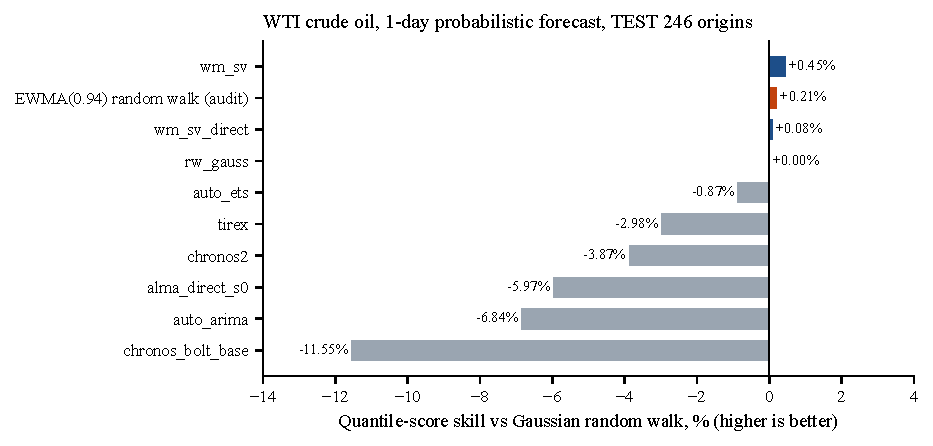
\includegraphics[width=0.78\linewidth]{figures/oil_skill.pdf}
\caption{Quantile-score skill vs the Gaussian random walk at $h=1$. The audit's EWMA(0.94) random walk, a volatility-only baseline, scores 0.010543 vs wm\_sv 0.010517 (\src{audit/oil\_check.csv}).}
\label{fig:oil}
\end{figure}

wm\_sv ranks first of 9 clean models at $h=1$, but its skill over the random walk is +0.45\% with $p=0.479$, which is a tie. It significantly beats only auto\_arima, Chronos-Bolt and Kronos-small. At $h=5$ and $h=20$ its skill is negative ($-0.76\%$ and $-0.53\%$). No model has a directional edge: at $h=1$, wm\_sv's direction accuracy is 0.492 against a majority rate of 0.549.

\subsection{German day-ahead power}
\begin{figure}[H]
\centering
\begin{subfigure}{0.49\linewidth}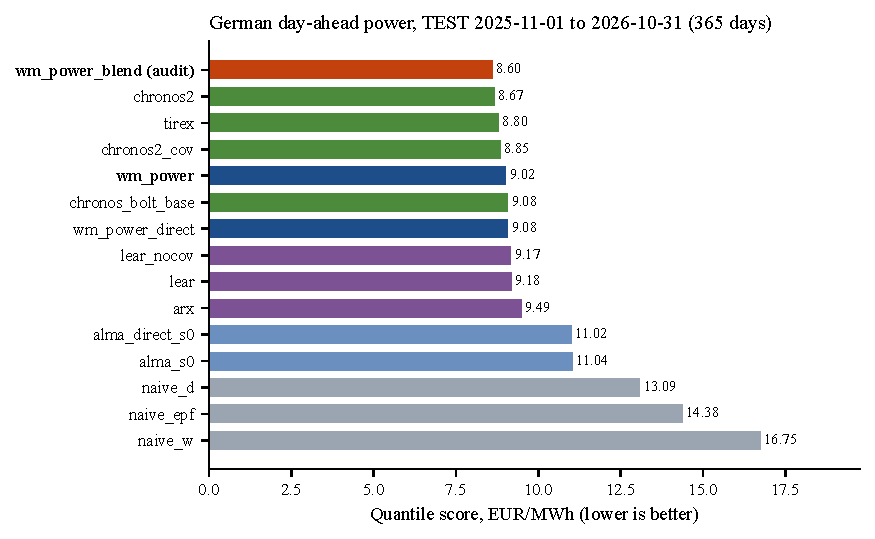
\includegraphics[width=\linewidth]{figures/power_qs.pdf}\end{subfigure}\hfill
\begin{subfigure}{0.49\linewidth}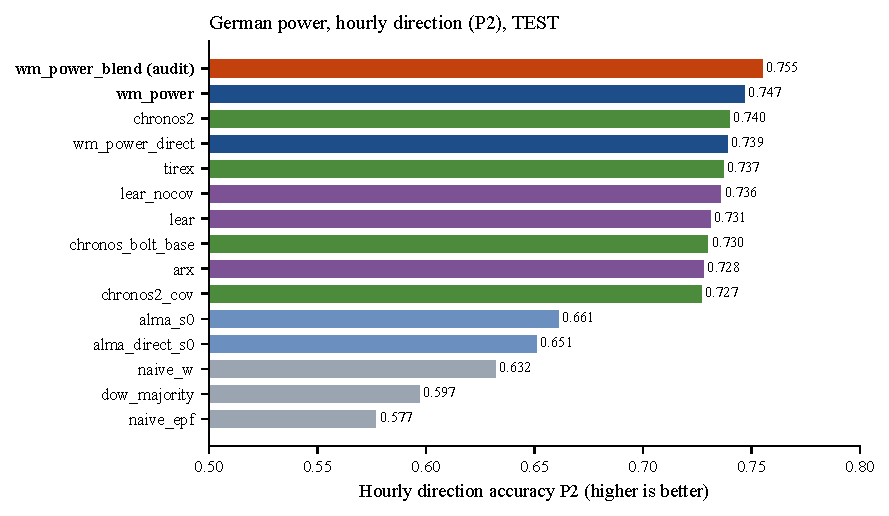
\includegraphics[width=\linewidth]{figures/power_p2.pdf}\end{subfigure}
\caption{Power, TEST year. Left: quantile score of the 24 hourly prices (lower is better). Right: hourly direction P2 (higher is better). Blue: Alma models; green: foundation models; purple: electricity-price (EPF) competitors; grey: naive baselines.}
\label{fig:power}
\end{figure}

\begin{table}[H]
\centering\small
\caption{Power: selected TEST results (\src{runs/power/test/report.md}; blend from \src{audit/validation/power\_blend.out}). The audit's scorer gives wm\_power QS 9.03 and MAE 22.44 on the same days, so blend comparisons use 9.03.}
\label{tab:power}
\begin{tabular}{@{}lccccc@{}}
\toprule
Model & P1 daily & P2 hourly & QS & MAE & cov80\\
\midrule
wm\_power & 0.732 & 0.747 & 9.02 & 22.43 & 0.752\\
wm\_power\_direct (twin) & 0.732 & 0.739 & 9.08 & 22.66 & 0.740\\
LEAR & 0.737 & 0.731 & 9.18 & 22.77 & 0.738\\
ARX & 0.740 & 0.728 & 9.49 & 23.35 & 0.793\\
Chronos-2 & 0.726 & 0.740 & \textbf{8.67} & 21.82 & 0.727\\
TiRex & 0.732 & 0.737 & 8.80 & 22.07 & 0.764\\
Zero-shot Alma (alma\_s0) & 0.668 & 0.661 & 11.04 & 27.22 & 0.703\\
\new{wm\_power\_blend} & \textbf{0.751} & \textbf{0.755} & \textbf{8.60} & \textbf{21.47} & --\\
\bottomrule
\end{tabular}
\end{table}

wm\_power is numerically first on hourly direction (0.747) but not significantly better than LEAR, ARX or the foundation models. It is fourth on quantile score, and its 80\% intervals under-cover (0.752). The repository notes a regime shift during TEST: prices doubled and 15-minute products were introduced.

\subsection{US natural-gas storage}
\begin{figure}[H]
\centering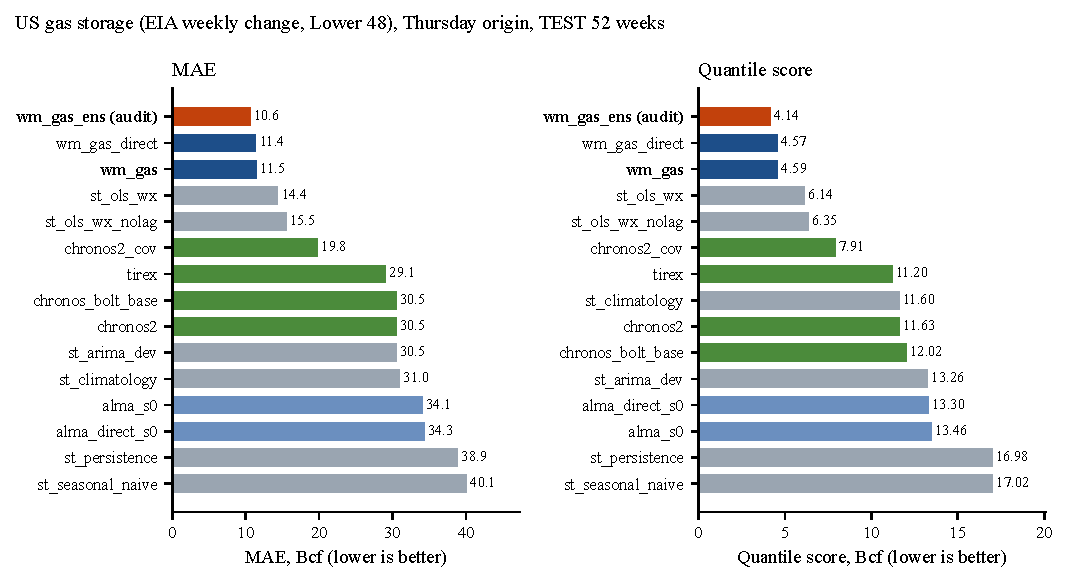
\includegraphics[width=\linewidth]{figures/gas_mae_qs.pdf}
\caption{Gas storage, Thursday origin, 52 TEST weeks. Left: MAE; right: quantile score (both lower is better).}
\label{fig:gas}
\end{figure}

wm\_gas has the best quantile score of all external models: it is significant vs OLS (Holm $p$ 0.030 Thursday, 0.039 Friday) and vs every foundation model. On MAE it beats every clean foundation model (11.5 vs Chronos-2 with covariates 19.8\,Bcf, Holm $p=0.0016$) but not OLS (14.4\,Bcf, $p=0.13$). Its direction accuracy (0.788) is below its own direct twin (0.865) and OLS (0.808).

\subsection{Crypto volatility (Alma-Fin)}
\begin{figure}[H]
\centering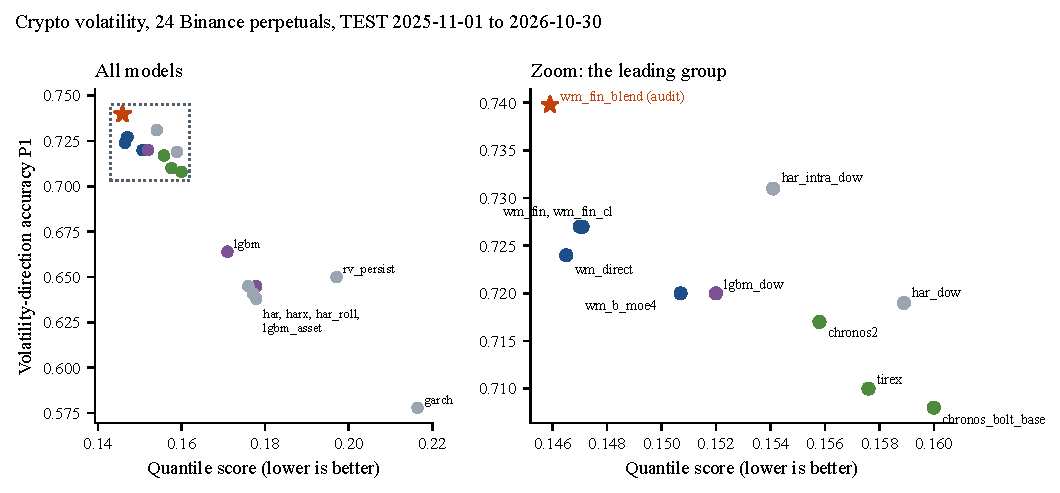
\includegraphics[width=\linewidth]{figures/fin_scatter.pdf}
\caption{Crypto, 24 coins: direction accuracy P1 against quantile score. The best models sit at the top left.}
\label{fig:fin}
\end{figure}

\begin{table}[H]
\centering\small
\caption{Crypto: TEST results for all 24 coins and the 8 held-out coins (\src{runs/fin/test/report.md}).}
\label{tab:fin}
\begin{tabular}{@{}lcccc@{}}
\toprule
& \multicolumn{2}{c}{All 24 coins} & \multicolumn{2}{c}{8 held-out coins}\\
\cmidrule(lr){2-3}\cmidrule(lr){4-5}
Model & P1 & QS & P1 & QS\\
\midrule
har\_intra\_dow (weekday HAR) & 0.731 & 0.1541 & 0.731 & 0.1569\\
wm\_fin & 0.727 & 0.1471 & 0.727 & 0.1496\\
wm\_direct (twin) & 0.724 & \textbf{0.1465} & 0.725 & 0.1489\\
lgbm\_dow & 0.720 & 0.1520 & 0.713 & 0.1555\\
Chronos-2 & 0.717 & 0.1558 & 0.718 & 0.1618\\
TiRex & 0.710 & 0.1576 & 0.711 & 0.1636\\
Chronos-Bolt & 0.708 & 0.1600 & 0.704 & 0.1669\\
lgbm\_asset (no weekday input) & 0.645 & 0.1779 & 0.647 & 0.1828\\
har\_roll (no weekday input) & 0.638 & 0.1779 & 0.635 & 0.1814\\
\new{wm\_fin\_blend} & \textbf{0.740} & 0.1459 & \textbf{0.741} & \textbf{0.1483}\\
\bottomrule
\end{tabular}
\end{table}

wm\_fin significantly beats Chronos-2, TiRex and Chronos-Bolt on quantile score (Holm $p$ 0.023, 0.002 and 0.0002, as reported by the project). On direction it ties the weekday-aware HAR (0.727 vs 0.731, $p=0.70$). On held-out coins it beats the baselines that lack a weekday input by 8--9 percentage points, but it does not beat har\_intra\_dow. The trading pillar failed: on held-out coins the world-model agent's net Sharpe was $-0.52$, against PPO $-0.27$ and DQN $+1.05$, so DQN is better ($p=0.025$). On 13 US ETFs, zero-shot direction was 0.582, below lgbm\_asset (0.603) and har\_roll (0.602).

% ================================================================== 7
\section{The world-model hypothesis}
\label{sec:wm}

\begin{figure}[H]
\centering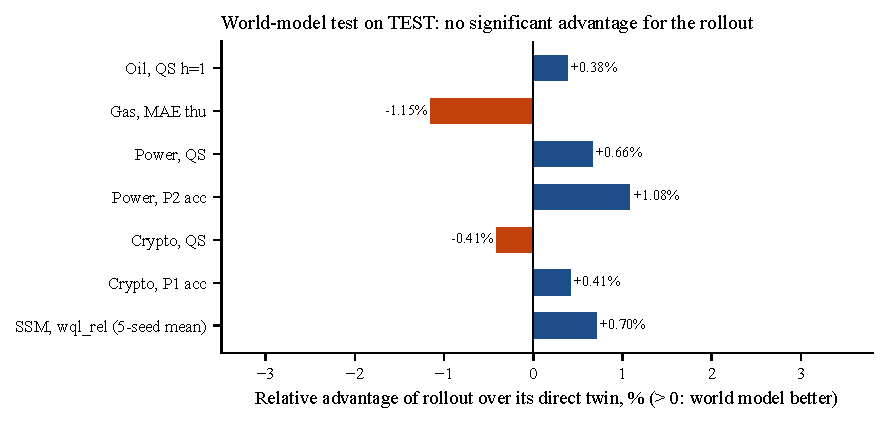
\includegraphics[width=0.8\linewidth]{figures/wm_test.pdf}
\caption{Relative advantage of each rollout model over its matched direct twin on TEST (positive means the world model is better). The sign varies across projects, and no project shows a significant advantage for the rollout (TEST reports, model cards and \cref{tab:ssm}). Gas MAE uses the audit's three-decimal values.}
\label{fig:wmtest}
\end{figure}

In every project the direct twin, which shares modules, parameter count, data, steps and seeds but has no rollout, is equal or better within noise. The power P2 rollout difference has raw $p=0.0168$ but fails Holm correction. The crypto rollout gain on P1 is +0.27 pp ($p=0.30$).

\paragraph{Research-track SSM over five seeds.} The research-program document claimed that the SSM family ``is the first to pass the WM test'', based on seed 0 alone. Seed 0 is also the seed that selected the SSM family. The direct twins for seeds 1--4 had never been trained, so the audit trained all 8 missing runs with the exact stored recipe (2,500 steps; SYN3/SYN5 synthetic data, curriculum 0.9, synthetic fraction 0.3, augmentation 0.5, GIFT\_CLEAN corpus).

\begin{figure}[H]
\centering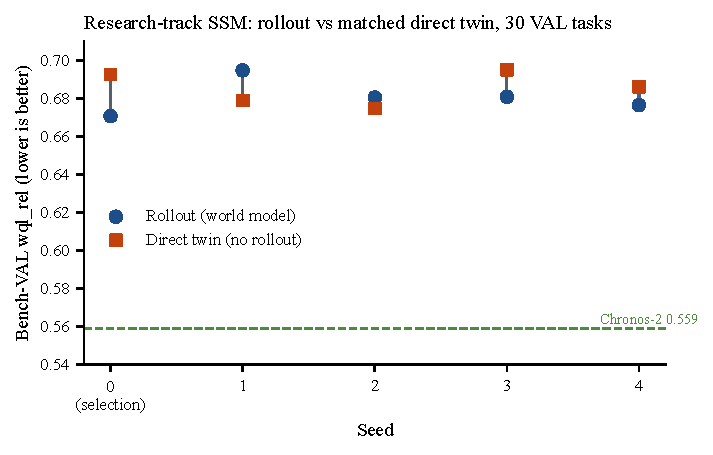
\includegraphics[width=0.72\linewidth]{figures/ssm_seeds.pdf}
\caption{SSM rollout vs its direct twin, bench-VAL wql\_rel (30 tasks, geometric mean vs Seasonal Naive; lower is better).}
\label{fig:ssm}
\end{figure}

\begin{table}[H]
\centering\small
\caption{Five-seed world-model test (\src{audit/ssm\_wm\_test.csv}; \src{audit/validation/ssm\_analysis.out}).}
\label{tab:ssm}
\begin{tabular}{@{}lccccc@{}}
\toprule
Seed & Rollout (re-run) & Published & Direct twin & Direct $-$ rollout & Tasks where rollout better\\
\midrule
0 (selection) & 0.6706 & 0.6707 & 0.6926 & +0.0220 & 24 / 30\\
1$^{*}$ & 0.6947 & 0.6936 & 0.6789 & $-$0.0158 & 17 / 30\\
2 & 0.6804 & 0.6804 & 0.6746 & $-$0.0059 & 16 / 30\\
3 & 0.6808 & 0.6808 & 0.6951 & +0.0143 & 16 / 30\\
4 & 0.6765 & 0.6765 & 0.6861 & +0.0096 & 17 / 30\\
\bottomrule
\end{tabular}
\par\smallskip\footnotesize $^{*}$Seed-1 runs were interrupted at about 1,500 steps and resumed from their checkpoints.
\end{table}

The rollout is better on 3 of 5 seeds. The mean per-task $\log(\text{direct}/\text{rollout})$ is $+0.0071$ (about 0.7\%), with family-cluster 95\% CI $[-0.0003, +0.0130]$: not significant. Excluding the selection seed, the mean is $+0.0008$, i.e.\ no effect. \textbf{The SSM does not pass the world-model test.}

% ================================================================== 8
\section{Zero-shot research track and public benchmarks}
\label{sec:research}

\begin{figure}[H]
\centering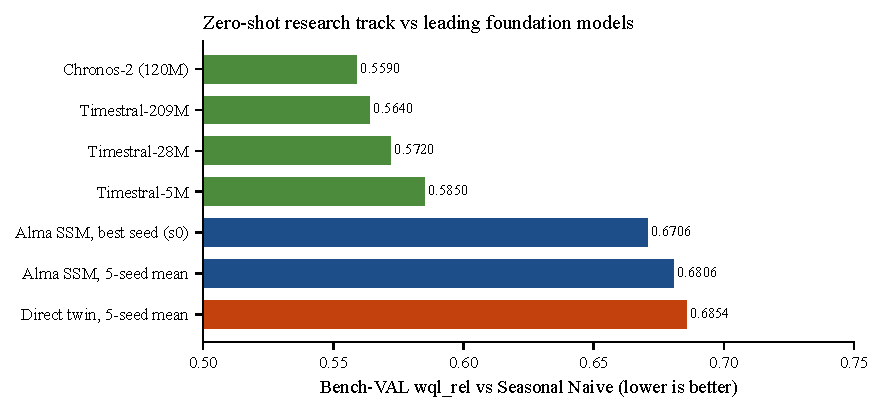
\includegraphics[width=0.8\linewidth]{figures/bench_val.pdf}
\caption{Internal bench-VAL (30 tasks, 13 families). Leaderboard models are as recorded in \src{docs/almats\_research\_program.md}; Alma values are from the audit re-runs.}
\label{fig:bench}
\end{figure}

On the internal bench-VAL, Alma's 5-seed mean of 0.6806 is 21.8\% worse than Chronos-2 (0.559) and 16.3\% worse than Timestral-5M (0.585). The project's own gap diagnosis attributes the gap of about 0.12 mainly to model capacity, context length, long-horizon decoding and calibration details. Note that the 30 VAL tasks were used for model selection (about 60 configurations were screened on them).

\paragraph{fev-bench status (PARTIAL).} The official fev-bench aggregation was reproduced exactly from the leaderboard result files (44 models, fev 0.10.0); see \cref{tab:fev}. Alma itself has \emph{no} fev-bench score yet. The 48 sealed TEST tasks were never exported. Of the 52 eligible non-TEST tasks, 47 were exported, 7 were predicted and 3 were smoke-scored before the run was paused, because the training process was using about 9.7\,GB on the 8\,GB machine. Twelve of the 52 tasks are self-flagged as overlapping the training data and would be replaced by Chronos-Bolt's scores under the fev rule.

\begin{table}[H]
\centering\small
\caption{fev-bench leaderboard (full 100 tasks) reproduced with the official code (\src{docs/fev\_full\_results.md}).}
\label{tab:fev}
\begin{tabular}{@{}lccc@{}}
\toprule
Model & SQL skill & MASE skill & WQL skill\\
\midrule
Timestral-209M & 50.39 & 39.49 & 54.63\\
Chronos-2 & 47.28 & 35.50 & 51.52\\
Timestral-5M & 46.19 & 34.54 & 50.49\\
TiRex & 42.58 & 30.01 & 46.67\\
Chronos-Bolt & 38.89 & 26.52 & 43.19\\
AutoTheta & 5.46 & 10.99 & 7.85\\
AutoETS & $-$26.82 & 2.26 & $-$27.03\\
Alma & \multicolumn{3}{c}{not yet scored}\\
\bottomrule
\end{tabular}
\end{table}

% ================================================================== 9
\section{Improvements made in the audit}
\label{sec:improve}

Every improvement followed the same discipline: start small on development data, scale only what helps, freeze the choice in writing, then look at TEST once.

\subsection{Selection algorithm}
\begin{algorithm}[H]
\caption{Leave-one-fold-out (LOFO) blend-weight selection on DEV}
\label{alg:lofo}
\KwIn{out-of-fold quantile forecasts $Q^{\text{nn}}_k$ (model pool) and $Q^{\text{b}}_k$ (simple baseline) for DEV folds $k=1..K$; weight grid $\mathcal{W}$}
\KwOut{fold-wise weights, used to check stability, and the final weight $w^\star$}
\For{$k \leftarrow 1$ \KwTo $K$}{
  $w_k \leftarrow \arg\min_{w\in\mathcal{W}} \sum_{j\neq k} \mathrm{MAE}\big(\mathrm{sort}((1-w)Q^{\text{nn}}_j + wQ^{\text{b}}_j)\big)$\;
  record the fold-$k$ score of $\mathrm{sort}((1-w_k)Q^{\text{nn}}_k + w_kQ^{\text{b}}_k)$ \tcp*{honest out-of-fold estimate}
}
$w^\star \leftarrow \arg\min_{w} \sum_{k}\mathrm{MAE}_k(w)$ \tcp*{full-DEV optimum; accepted only if all $w_k$ are close to it}
\end{algorithm}

\subsection{Gas storage: seed ensemble, OLS blend and adaptive intervals}
\begin{figure}[H]
\centering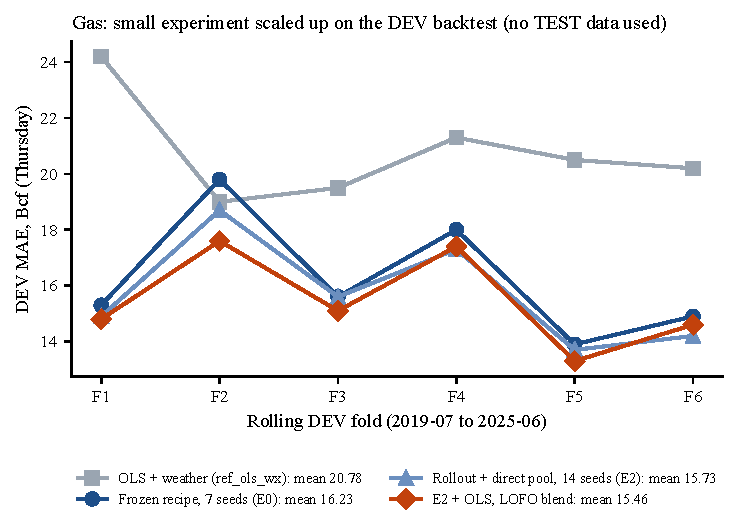
\includegraphics[width=0.78\linewidth]{figures/gas_dev_folds.pdf}
\caption{Gas DEV backtest (6 rolling folds, 2019-07 to 2025-06; Thursday origin). The audit trained 8 new backtest runs (seeds 3--6 of both recipes). The 14-member pool plus OLS (LOFO weights) has a lower MAE than the frozen recipe in all 6 folds: mean 15.46 vs 16.23\,Bcf (\src{audit/gas\_exp\_scaled.csv}). With the single full-DEV weight 0.2, which was frozen, the DEV MAE is 15.39 (Thursday) and 15.27 (Friday).}
\label{fig:gasdev}
\end{figure}

\begin{algorithm}[H]
\caption{wm\_gas\_ens forecast (as implemented in \src{repo/tools/gas/wm\_gas\_ens.py})}
\label{alg:gasens}
\KwIn{context at origin $t$; 14 members (wm\_gas and wm\_gas\_direct seeds 0--6); released errors of past weeks}
$Q^{\text{nn}} \leftarrow$ quantile-wise mean of the 14 members\;
$Q \leftarrow \mathrm{sort}(0.8\,Q^{\text{nn}} + 0.2\,Q^{\text{ols}})$ \tcp*{weather OLS baseline st\_ols\_wx}
$e \leftarrow$ mean absolute median error over the last 8 weeks \emph{released before} $t$\;
$s \leftarrow \mathrm{clip}\big((e/\mathrm{ref})^{0.5}, 0.4, 2.0\big)$, with ref $=15.39$ (Thursday) or $15.27$ (Friday), and $s=1$ if fewer than 4 past weeks\;
\Return{$\hat q_\tau = \mathrm{median} + s\,(Q_\tau - \mathrm{median})$} \tcp*{interval width adapts to recent error}
\end{algorithm}

\begin{figure}[H]
\centering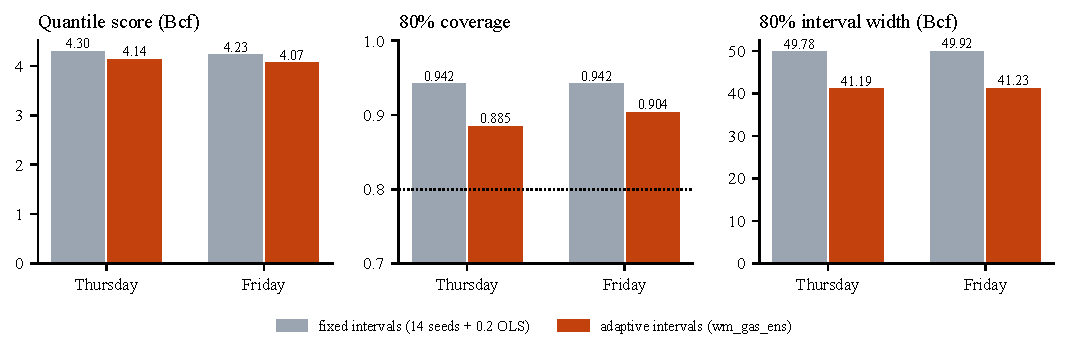
\includegraphics[width=0.92\linewidth]{figures/gas_intervals.pdf}
\caption{Effect of the adaptive interval rule on TEST (\src{audit/validation/gas\_final2.out}). The 80\% interval narrows by 17\% and coverage moves from 0.942 towards the nominal 0.80. A leak test that scrambles the global data store read by the interval step changed 0 of 22 wm\_gas\_ens forecasts (\src{audit/validation/gas\_ens\_leak.out}).}
\label{fig:gasint}
\end{figure}

\begin{table}[H]
\centering\small
\caption{Gas TEST, Lower 48, 52 weeks (\src{audit/validation/gas\_final.out} and \src{gas\_final2.out}).}
\label{tab:gasimp}
\begin{tabular}{@{}lcccc@{}}
\toprule
Model & MAE thu / fri (Bcf) & QS thu / fri & cov80 thu / fri & Direction thu / fri\\
\midrule
wm\_gas (frozen) & 11.53 / 11.56 & 4.59 / 4.56 & 0.865 / 0.885 & 0.788 / 0.808\\
wm\_gas\_direct (frozen) & 11.40 / 11.08 & 4.57 / 4.47 & 0.865 / 0.885 & 0.865 / 0.808\\
st\_ols\_wx (OLS + weather) & 14.35 / 14.46 & 6.14 / 6.09 & 0.827 / 0.846 & 0.808 / 0.808\\
14-seed pool + 0.2 OLS & 10.63 / 10.46 & 4.30 / 4.23 & 0.942 / 0.942 & 0.808 / 0.788\\
\new{wm\_gas\_ens} (+ adaptive intervals) & \textbf{10.63 / 10.46} & \textbf{4.14 / 4.07} & 0.885 / 0.904 & 0.808 / 0.788\\
\bottomrule
\end{tabular}
\end{table}

\begin{table}[H]
\centering\small
\caption{Gas paired bootstrap differences on TEST (pool + 0.2 OLS minus comparator; 4,000 replicates).}
\label{tab:gassig}
\begin{tabular}{@{}llccc@{}}
\toprule
Origin & Comparator & $\Delta$MAE [95\% CI] & $\Delta$QS [95\% CI] & Significant?\\
\midrule
Thursday & wm\_gas & $-0.90$ [$-2.54$, $+0.65$] & $-0.29$ [$-0.87$, $+0.20$] & \no\\
Friday & wm\_gas & $-1.11$ [$-2.72$, $+0.41$] & $-0.33$ [$-0.90$, $+0.14$] & \no\\
Thursday & st\_ols\_wx & $-3.72$ [$-6.99$, $-0.60$] & $-1.84$ [$-2.89$, $-0.87$] & \yes\\
Friday & st\_ols\_wx & $-4.00$ [$-7.29$, $-0.96$] & $-1.86$ [$-2.94$, $-0.89$] & \yes\\
Thursday & adaptive vs fixed intervals & -- & $-0.157$ [$-0.245$, $-0.065$] & \yes\\
Friday & adaptive vs fixed intervals & -- & $-0.161$ [$-0.244$, $-0.079$] & \yes\\
\bottomrule
\end{tabular}
\end{table}

\subsection{Power and crypto: quantile blends with the strongest simple baseline}
\begin{figure}[H]
\centering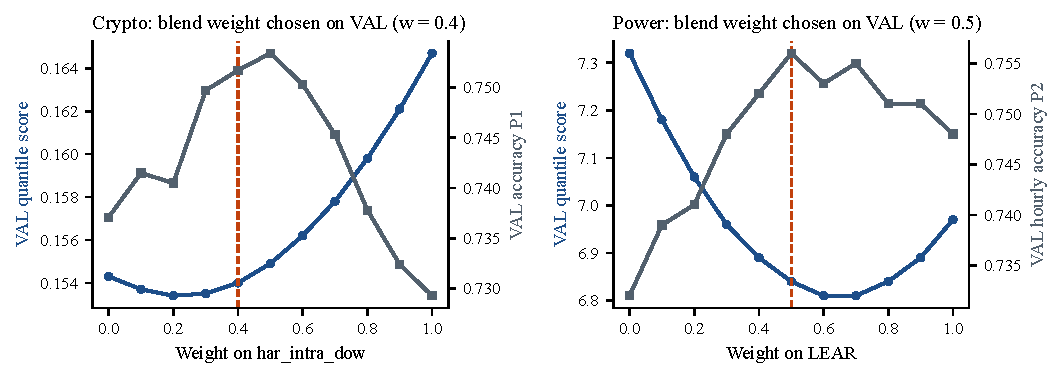
\includegraphics[width=\linewidth]{figures/val_weights.pdf}
\caption{Blend weights were chosen on VAL only (July to October 2025), before any TEST look (\src{audit/validation/fin\_blend.out}, \src{power\_blend.out}).}
\label{fig:valw}
\end{figure}

\begin{table}[H]
\centering\small
\caption{Blend results on TEST with block-bootstrap 95\% CIs (\src{audit/validation/power\_boot.out}, \src{fin\_boot.out}). Crypto accuracy is compared under the same median rule (wm\_fin 0.724 under that rule; 0.727 under its own probability rule).}
\label{tab:blend}
\resizebox{\linewidth}{!}{%
\begin{tabular}{@{}llccc@{}}
\toprule
Blend & Comparator & Metric & Difference [95\% CI] & Significant?\\
\midrule
\multirow{4}{*}{\shortstack[l]{\new{wm\_power\_blend}\\0.5 wm\_power + 0.5 LEAR}} & wm\_power & QS & $-0.426$ [$-0.674$, $-0.174$] & \yes\\
& wm\_power & P2 & $+0.0082$ [$-0.0033$, $+0.0194$] & \no\\
& LEAR & QS & $-0.619$ [$-0.900$, $-0.356$] & \yes\\
& LEAR & P2 & $+0.0250$ [$+0.0138$, $+0.0364$] & \yes\\
\midrule
\multirow{4}{*}{\shortstack[l]{\new{wm\_fin\_blend}\\0.6 wm\_fin + 0.4 har\_intra\_dow}} & wm\_fin & P1 & $+1.67$ pp [$+0.45$, $+2.92$] & \yes\\
& wm\_fin & QS & $-0.0014$ [$-0.0034$, $+0.0007$] & \no\\
& har\_intra\_dow & P1 & $+0.89$ pp [$-0.55$, $+2.34$] & \no\\
& har\_intra\_dow & QS & $-0.0082$ [$-0.0111$, $-0.0055$] & \yes\\
\bottomrule
\end{tabular}}
\end{table}

The crypto blend's result is not sensitive to the weight: for weights 0.3, 0.4 and 0.5 the direction gain over wm\_fin is +1.58, +1.67 and +1.86 pp, all with CIs excluding 0.

\subsection{Summary of improvements}
\begin{table}[H]
\centering\small
\caption{Improved models (packaged in \src{repo/winning\_models/} with sha256-checked wrappers).}
\label{tab:impsum}
\begin{tabularx}{\linewidth}{@{}lXX@{}}
\toprule
Model & TEST change vs the original model & Significance\\
\midrule
\new{wm\_gas\_ens} & MAE 10.63 vs 11.53 (Thursday, $-7.8\%$); QS 4.14 vs 4.59 & Significant vs OLS on MAE and QS; not significant vs wm\_gas\\
\new{wm\_power\_blend} & QS 8.60 vs 9.03 ($-4.8\%$); P2 0.755 vs 0.746 & QS significant vs both members; P2 significant vs LEAR only\\
\new{wm\_fin\_blend} & P1 0.740 vs 0.724 (same rule); QS 0.1459 vs 0.1471 & P1 significant vs wm\_fin; not significant vs har\_intra\_dow on P1\\
Oil & No improvement attempted & The model is indistinguishable from a random walk, so there is no signal to add\\
\bottomrule
\end{tabularx}
\end{table}

% ================================================================== 10
\section{Corrections to published claims}
\label{sec:claims}
\begin{table}[H]
\centering\small
\caption{Claims corrected in \src{README.md}, \src{winning\_models/README.md}, the model cards and \src{docs/almats\_research\_program.md}.}
\label{tab:claims}
\begin{tabularx}{\linewidth}{@{}p{4.2cm}Xp{1.7cm}@{}}
\toprule
Original claim & Evidence & Action\\
\midrule
Crypto ``transfers to unseen coins, +8--9 pp, Holm $<10^{-4}$'' & Measured only against baselines without a weekday input; har\_intra\_dow scores 0.731 vs wm\_fin 0.727 on the held-out coins & Corrected\\
Oil ``wm\_sv ranks \#1 of 9'' & Skill +0.45\%, $p=0.479$; an EWMA random walk scores 0.010543 vs 0.010517 & Corrected\\
SSM ``first to pass the world-model test'' & Seed 0 only; over 5 seeds the gain is not significant (+0.08\% without seed 0) & Corrected\\
World model drives the gains & Direct twin equal or better in all projects & Disclosed\\
Older research leaderboard (38 numbers) & The repository's own audit\_v3 says none is traceable to code and config & Noted\\
\bottomrule
\end{tabularx}
\end{table}

% ================================================================== 11
\section{Engineering changes}
\label{sec:engineering}

\subsection{Forward test}
\begin{algorithm}[H]
\caption{Forward test with a frozen-hash guard (\src{repo/tools/forward/forward\_eval.py})}
\label{alg:fwd}
\textbf{freeze} (run once, 2026-11-01 17:47 UTC): record the sha256 of 29 code and checkpoint files in \src{FREEZE.json}\;
\textbf{refresh}: download newly published public data (EIA, CPC, Energy-Charts, Binance)\;
\textbf{score}: \lIf{any pinned file's sha256 differs}{refuse to run}
for each project, forecast and score only target periods after \texttt{FORWARD\_START} = 2026-11-02\;
compare wm\_gas\_ens, wm\_gas, wm\_gas\_direct and st\_ols\_wx (gas); wm\_power\_blend, wm\_power and LEAR (power); and wm\_fin\_blend, wm\_fin and har\_intra\_dow (crypto)\;
\end{algorithm}

\subsection{Reproducibility}
Training is bit-identical run to run on the same machine; the audit measured a difference of exactly 0.0. The small drift against the original checkpoints comes from different hardware (multithreaded floating-point sums). A new switch, \texttt{ALMA\_THREADS=1}, in all trainers gives single-threaded, deterministic training across machines (oil reproduced across machines to $7\times10^{-7}$). The default behaviour is unchanged, which was verified bit-identical. Documented in \src{docs/reproducibility.md}.

\subsection{Repository changes}
The merge into \texttt{main} (\texttt{43b463b}) changed 36 files, adding 699 lines and modifying 13. It contains two commits: \texttt{9f96b36} (claim corrections, three new models with cards and checkpoints, forward test, reproducibility switch) and \texttt{7f8c068} (5-seed SSM test and the research-doc correction). Raw data and audit checkpoints were not committed.

% ================================================================== 12
\section{Project 5: Alma-Live Gas (in progress)}
\label{sec:live}
The live project's goal is UNG forecasting and paper trading with continual learning (\src{docs/live\_gas\_research.md}). Verified state on 3 November 2026:
\begin{itemize}
\item A harness and data pins exist. Historical baselines were scored on DEV and on VAL (332 days, 2024-07-01 to 2025-10-24); the harness labels history as \emph{not} the claim test.
\item Eight shadow paper-trading ledgers (buy\_hold, short\_ung\_carry, tsmom\_20, seasonal, weather\_rev, storage\_surprise, fc\_ewma and fc\_hist) were initialised on 2026-11-01 with genesis entries only.
\item The world-model search protocol (\src{docs/live\_search.md}) was committed with amendments A1--A3 before any DEV score. No world-model result is recorded in the repository.
\item The project's own research brief states that storage-forecast skill gave no price edge in the earlier gas study (hit rates 0.47 and 0.50), and that 12 months of daily paper trading can only detect an annual Sharpe of about 1.65 at 50\% power.
\end{itemize}

% ================================================================== 13
\section{Targets, projections and time to confirmation}
\label{sec:projection}

\subsection{How long until the improvements can be confirmed}
The forward test scores only new data, so its length is set by how quickly data arrive. \Cref{tab:proj} estimates the forward sample needed to confirm each improvement, assuming the TEST-year effect size and variability persist. For a paired difference with TEST mean $d$ and bootstrap 95\% CI $[l,u]$ on $n$ units, $\mathrm{SE}=(u-l)/3.92$ and the per-unit standard deviation is $\mathrm{SE}\sqrt{n}$; the sample needed for a two-sided 5\% test at 80\% power is $n^\star=\big(2.80\cdot \mathrm{SE}\sqrt{n}/|d|\big)^2$. These are planning approximations, not guarantees: if an effect shrinks out of sample, the required time grows.

\begin{table}[H]
\centering\small
\caption{Forward sample needed for 80\% power (\src{audit/validation/projections.out}).}
\label{tab:proj}
\begin{tabular}{@{}lllrr@{}}
\toprule
Improvement & Comparison & TEST result & $n^\star$ & Approx.\ time\\
\midrule
Gas MAE (Thursday) & vs st\_ols\_wx & significant & 78 weeks & 1.5 years\\
Gas MAE (Thursday) & vs wm\_gas & not significant & 333 weeks & 6.4 years\\
Power QS & vs LEAR & significant & 144 days & 0.4 years\\
Power QS & vs wm\_power & significant & 256 days & 0.7 years\\
Power P2 & vs wm\_power & not significant & 1,427 days & 3.9 years\\
Crypto QS & vs har\_intra\_dow & significant & 87 days & 0.2 years\\
Crypto P1 & vs wm\_fin & significant & 406 days & 1.1 years\\
Crypto P1 & vs har\_intra\_dow & not significant & 1,958 days & 5.4 years\\
\bottomrule
\end{tabular}
\end{table}

\begin{table}[H]
\centering\small
\caption{Forward-test calendar (EIA reports are normally on Thursdays; holiday weeks can shift by a day).}
\label{tab:calendar}
\begin{tabular}{@{}ll@{\hspace{2cm}}ll@{}}
\toprule
Gas release & Date & Power/crypto day & Date\\
\midrule
\#1 & 2026-11-05 & 30 & 2026-12-01\\
\#13 & 2027-01-28 & 60 & 2026-12-31\\
\#20 & 2027-03-18 & 180 & 2027-04-30\\
\#52 & 2027-10-28 & 365 & 2027-11-01\\
\bottomrule
\end{tabular}
\end{table}

\paragraph{Reading the projection.} The comparisons that were already significant on TEST could be confirmed in roughly 3 months (crypto QS vs har\_intra\_dow) to 1.5 years (gas vs OLS). Gains over the original Alma models on point accuracy or direction are small relative to the noise; confirming them would take several years, so the improvements are best described as consistent but modest.

\subsection{Targets for the research track}
\begin{table}[H]
\centering\small
\caption{Research-track position against its targets (bench-VAL wql\_rel, lower is better). The ceiling and target rows are the project's own stated estimates (\src{docs/almats\_research\_program.md}), not measured results.}
\label{tab:targets}
\begin{tabularx}{\linewidth}{@{}Xlp{4.6cm}@{}}
\toprule
Item & Value & Type\\
\midrule
Alma SSM today, 5-seed mean (best seed) & 0.6806 (0.6706) & measured\\
Timestral-5M / Timestral-28M / Timestral-209M & 0.585 / 0.572 / 0.564 & reported\\
Chronos-2 & 0.559 & reported\\
``Realistic ceiling'' on the 8\,GB Mac with a 1--5M model & 0.59--0.62 & project's speculative estimate\\
Pre-registered target (10\% better than the best baseline) & $\leq$0.503 & target; the project notes that no published model of $\leq$10M parameters supports it\\
\bottomrule
\end{tabularx}
\end{table}

\paragraph{Time estimates stated in the repository.}
\begin{itemize}
\item \textbf{fev-bench completion:} the remaining seed-0 predictions were estimated at about 40--60 minutes on an unloaded machine, plus about the same per extra seed, followed by scoring and aggregation (\src{docs/fev\_full\_results.md}). This must run on an unloaded machine, because the pause happened under memory pressure.
\item \textbf{Scaling:} the goal document budgets about 1--3 nights per 5M-parameter training run on the Mac.
\item \textbf{Alma-Live:} about 2--4 weeks for the extended world model, audits and freeze, and about 12--24+ months for statistical confirmation of trading P\&L (\src{docs/live\_gas\_research.md}).
\end{itemize}

\subsection{Recommended next steps}
\begin{enumerate}
\item Run the forward-test \texttt{refresh} and \texttt{score} commands weekly from 5 November 2026, and report results only at the pre-set checkpoints in \cref{tab:calendar}.
\item Finish fev-bench on the 52 eligible tasks on an unloaded machine, reporting the nonval22 subset alongside the full set, so that the project has its first public-benchmark number.
\item Treat the world-model claim as unsupported. Either redesign the model so that the rollout is the only path to the future (as the project's research program proposes) or reposition the models as strong state-space forecasters.
\item For Alma-Live, keep the forecasting endpoints as the headline claims, since the sample can support them, and report P\&L as secondary until about two years of data exist.
\end{enumerate}

% ================================================================== 14
\section{Limitations and threats to validity}
\begin{itemize}
\item \textbf{Second look at TEST.} The audit models were scored on a TEST year the project had already scored. All choices were fixed on DEV/VAL first, but some winner's-curse risk remains; the forward test is the real check.
\item \textbf{Small samples.} Gas has 52 TEST weeks, so many differences of about 1\,Bcf are not significant.
\item \textbf{Selection exposure.} The research bench's 30 VAL tasks were used for tuning. The crypto universe was ranked on VAL-period volume, and the held-out coins were used during selection.
\item \textbf{Data drift.} Some rebuilt files differ from their pins (\cref{tab:verify}). The reproduced headline numbers are unaffected, but ETF and oil-inventory results were not re-verified.
\item \textbf{Repo-reported statistics.} Holm $p$-values for the original models are taken from the project's TEST reports and model cards. The audit recomputed the scores, not every $p$-value.
\item \textbf{Projection assumptions.} \Cref{tab:proj} assumes that effects and variability persist and ignores changes in autocorrelation.
\end{itemize}

% ================================================================== 15
\section{Conclusion}
The Alma project is honestly built and honestly evaluated: an independent rebuild found no leakage and no fabricated numbers. Its strongest verified result is in US gas storage, where the original model has the best probabilistic score among all external models and the audit ensemble lowers MAE to 10.63\,Bcf. The project's defining hypothesis, that learned latent rollouts beat direct decoding, is not supported by any experiment so far. On the zero-shot track Alma remains about 16--22\% behind the leading small and medium foundation models, and it has no public-benchmark score yet. The improved models are frozen and will be judged on new data from 5 November 2026. Improvements over simple baselines that were already significant could be confirmed within months; small gains over the original models will take years.

\appendix
% ================================================================== A
\section{Provenance of numbers}
\label{app:provenance}
\begin{longtable}{@{}p{5.2cm}p{9.6cm}@{}}
\toprule
Numbers & Source file\\
\midrule
\endhead
Oil TEST tables & \src{repo/runs/commodity/test/report\_wm\_sv.md}\\
Power TEST tables & \src{repo/runs/power/test/report.md}\\
Gas TEST tables & \src{repo/runs/gas/test/report.md}\\
Crypto TEST tables, agents, ETF & \src{repo/runs/fin/test/report.md}\\
Original-model Holm $p$-values & \src{repo/winning\_models/*/MODEL\_CARD.md}\\
Leak tests (re-run 3 Nov) & \src{audit/validation/\{oil,gas,power\}\_check.out}, \src{gas\_ens\_leak.out}\\
Oil EWMA baseline & \src{audit/oil\_check.csv}\\
Gas DEV experiments & \src{audit/gas\_exp.csv}, \src{audit/gas\_exp\_scaled.csv}\\
Gas TEST improvement and CIs & \src{audit/validation/gas\_final.out}, \src{gas\_final2.out}\\
Power blend and CIs & \src{audit/validation/power\_blend.out}, \src{power\_boot.out}\\
Crypto blend and CIs & \src{audit/validation/fin\_blend.out}, \src{fin\_boot.out}, \src{audit/fin\_score.csv}\\
SSM 5-seed test & \src{audit/ssm\_wm\_test.csv}, \src{audit/validation/ssm\_analysis.out}, \src{audit/logs/aud\_ssm\_*.log}\\
Bench-VAL leaderboard values, targets & \src{repo/docs/almats\_research\_program.md}\\
fev-bench status and leaderboard & \src{repo/docs/fev\_full\_results.md}\\
Goal, tiers, leaderboard targets & \src{repo/alma\_goal.md}\\
Alma-Live status & \src{repo/docs/live\_*.md}, \src{repo/runs/live/}\\
Forward-test freeze & \src{repo/tools/forward/FREEZE.json}\\
Projections and calendar & \src{report/projections.py}, \src{audit/validation/projections.out}\\
Every plotted value & \src{report/make\_figures.py}, \src{report/facts.json}\\
\bottomrule
\end{longtable}

% ================================================================== B
\section{Reproduction commands}
\begin{verbatim}
# audit re-runs (from the audit folder; repo virtual environment)
python oil_check.py ; python gas_check.py ; python power_check.py
python gas_final.py --ckpts wm_gas,wm_gas_direct,x_wm_s3456,x_dir_s3456 --w-ols 0.2
python gas_final2.py ; python power_blend.py ; python power_boot.py
python fin_blend.py ; python fin_boot.py ; python ssm_analysis.py
# report
python report/projections.py ; python report/make_figures.py
# forward test (from the repo)
python tools/forward/forward_eval.py refresh
python tools/forward/forward_eval.py score
\end{verbatim}

% ================================================================== C
\section{Glossary}
\begin{description}[leftmargin=3.2cm,style=nextline,itemsep=1pt]
\item[World model] A model that encodes history into a latent state and advances it step by step with a learned transition; forecasts are read from the simulated states.
\item[Direct twin] The same model, decoding the whole horizon at once without a rollout; the control in the world-model test.
\item[QS] Quantile score (mean pinball loss); lower is better.
\item[wql\_rel] Weighted quantile loss relative to Seasonal Naive, geometric mean over tasks; lower is better.
\item[SQL skill] fev-bench scaled quantile loss skill vs Seasonal Naive, in percent; higher is better.
\item[DEV / VAL / TEST] Development data for selection, validation for checks, and the sealed TEST year scored once.
\item[LOFO] Leave-one-fold-out: a choice is made on all folds but one and scored on the held-out fold.
\item[Holm correction] Adjusts $p$-values for multiple comparisons.
\item[Forward test] Scoring frozen models only on data published after they were frozen.
\end{description}

\end{document}
